% !TeX root = solutions_main.tex
\section*{Task 1: Solution}
\begin{enumerate}[label=\alph*)]
    \item\label{item:task1a} The solution computed by \lstinline|ode45| is incorrect. The second component should have a bend when the first component crosses the $750$ threshold.

	The integrator \lstinline|ode45| can only be used to solve smooth systems. The switched system, however, contains discontinuities in the RHS. Since the system violates a key requirement of \lstinline|ode45|, we cannot expect to receive a correct solution. The integrator \lstinline|ode45| is simply not designed to solve these types of switched problems.
	
	For this particular example, the integrator takes large steps because the system is smooth at the beginning. Due to the large step size, the integrator completely misses the discontinuity (which it has no way of knowing about since the RHS is assumed to be smooth).\\\\
    \textbf{File:} \texttt{rhsTask1.m}
    \begin{lstlisting}
function dy = rhsTask1(t, y, p)
dy = zeros(2, 1);

q1 = 50/27*t^2 - 100/3*t + 400/3;
q2 = (1000-y(2)) * (p(1)*(t-19) + p(2));

if y(1) <= 750
    dy(1) = q1;
    dy(2) = 0;
elseif y(1) < 800
    dy(1) = q1 - q2;
    dy(2) = -300;
else
    dy(1) = q1 - q2;
    dy(2) = 0;
end
end
    \end{lstlisting}
    \textbf{File:} \texttt{runTask1.m}
    \begin{lstlisting}
%% Subtask a) and b)
%% Setup problem
tspan = [0, 30];
y0 = [0; 1000];
p = [3/4, 1/4];

rhs = @rhsTask1a;
integrator = @ode45;
optionsOde45 = odeset('RelTol', 1e-8, 'AbsTol', 1e-8);

%% Solve with ode45
solutionOde45 = integrator(@(t, y) rhs(t, y, p), tspan, y0, optionsOde45);

%% Plot solution
t = linspace(tspan(1), tspan(end), 1000);
yOde45 = deval(solutionOde45, t);

figure;
plot(t, yOde45);
title('Solution with ode45');
    \end{lstlisting}
    \begin{figure}[H]
        \centering
        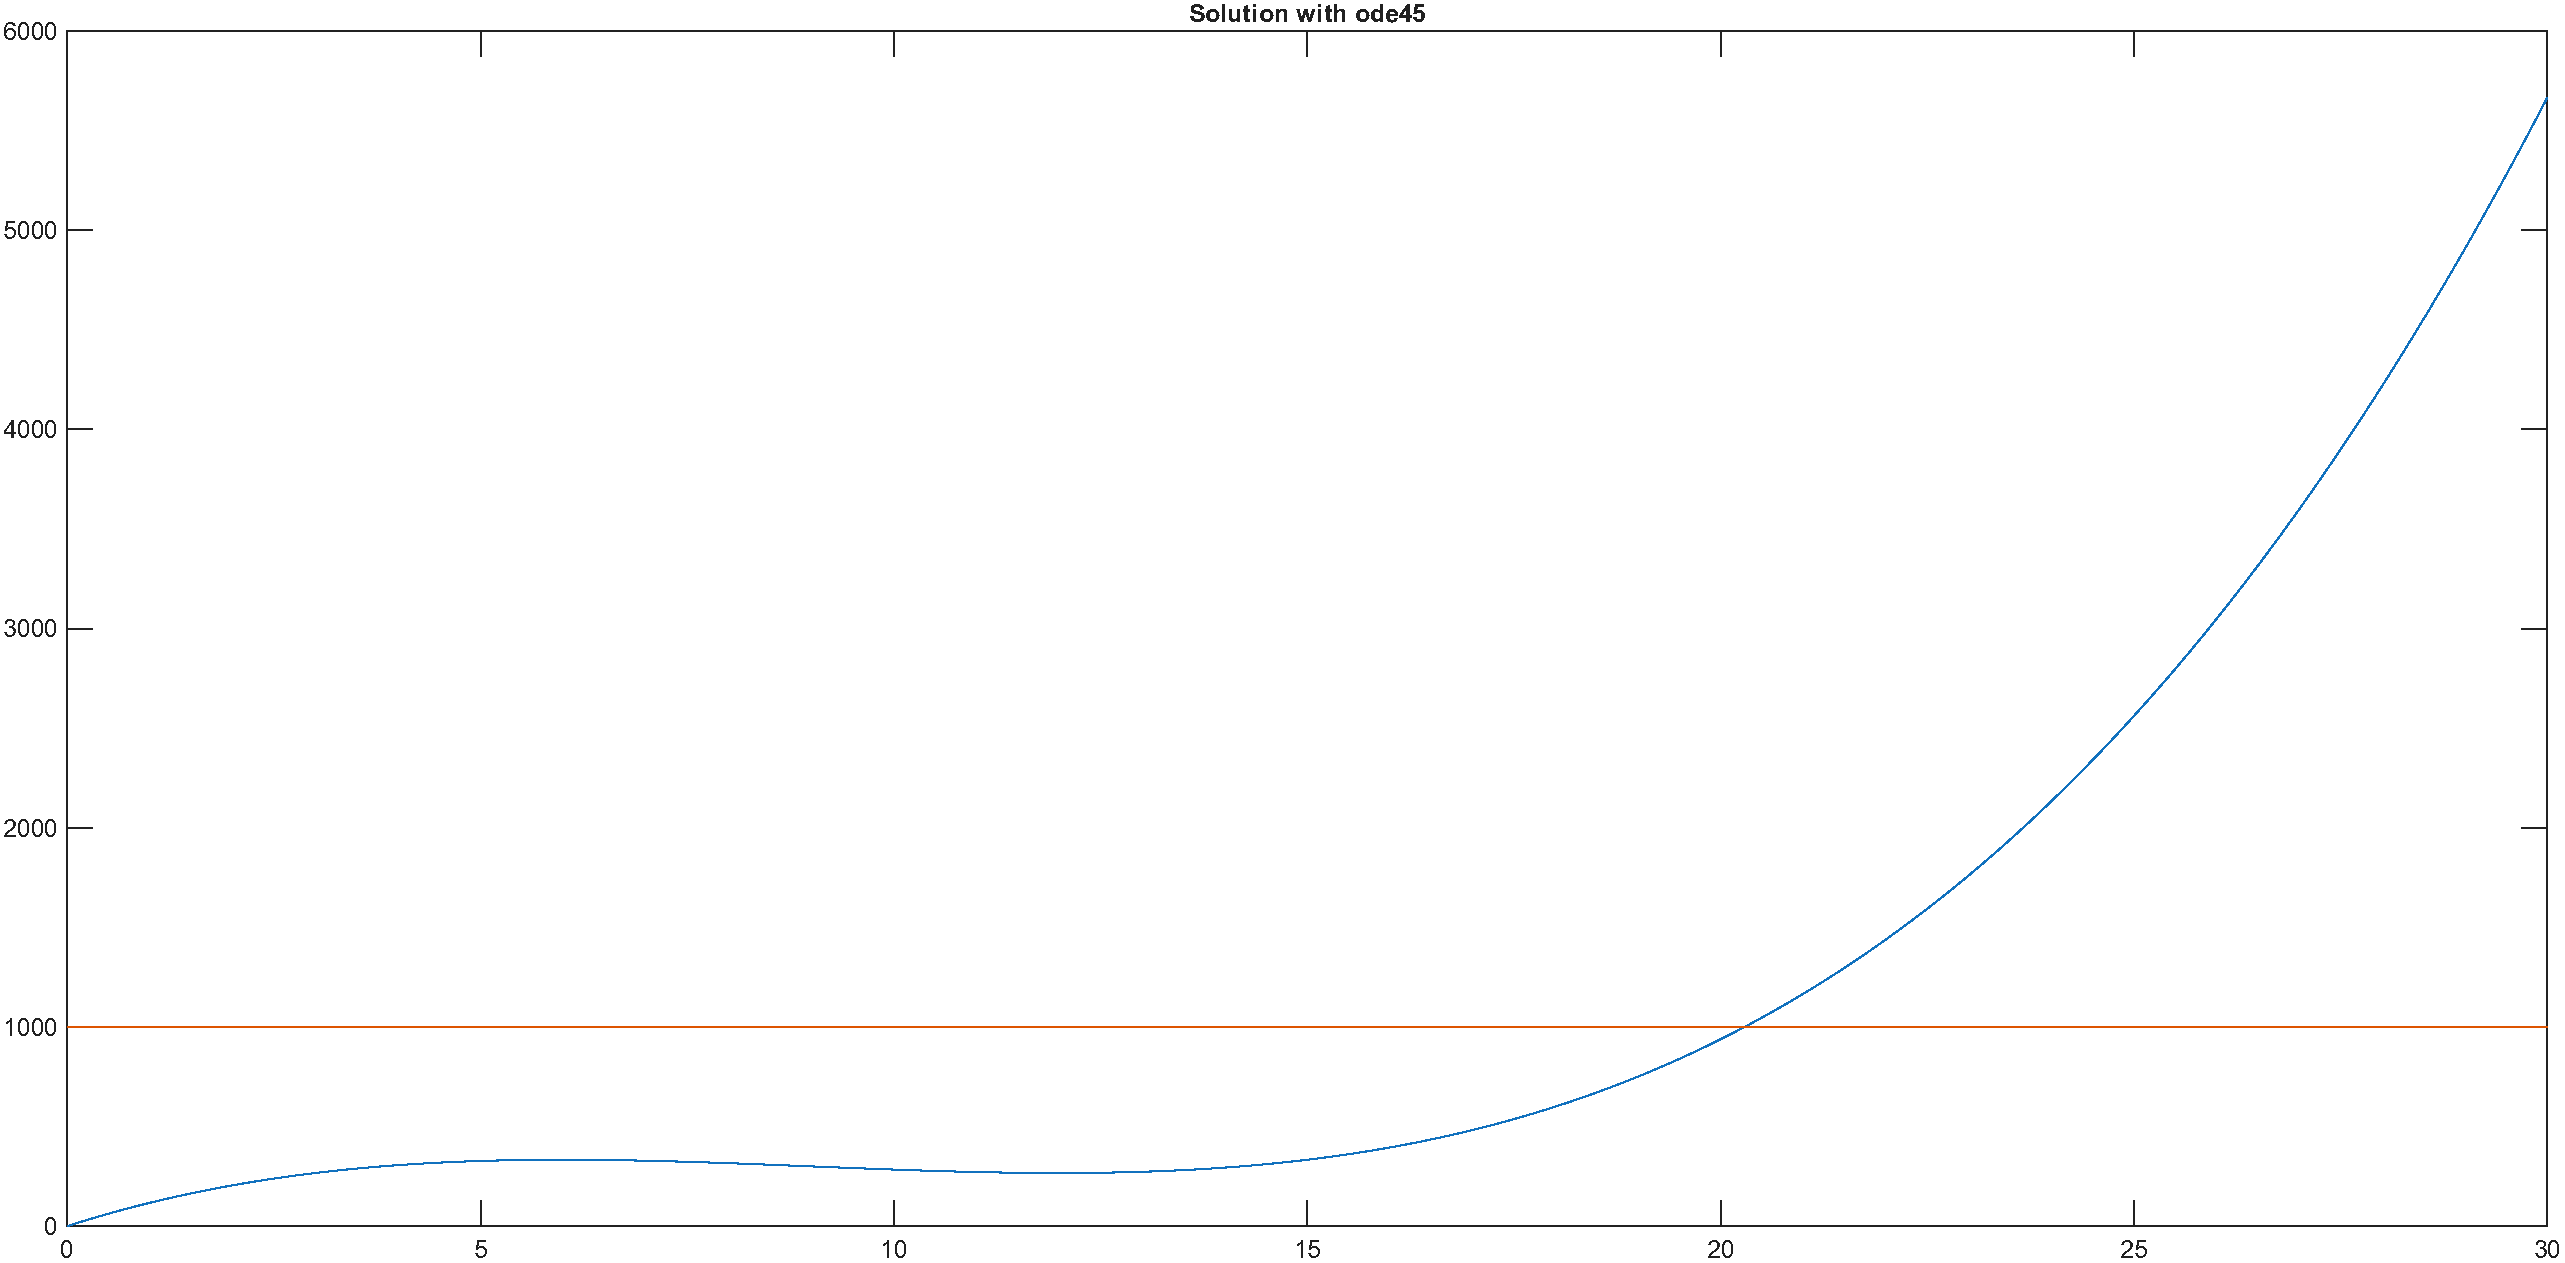
\includegraphics[width=\textwidth]{Plots/task1a}
        \caption{\textbf{Incorrect} solution plot with ode45 for subtask \ref{item:task1a}}
    \end{figure}

    \item\label{item:task1b} The solution produced by \lstinline|ode45| with a maximum integration step size of $0.1$ is correct. We can see the characteristic bend of the second solution component which was missing in the plot from subtask \ref{item:task1a}.
	
	By forcing the integrator to take tiny steps, it manages to approximate the non-smooth regions of the solution through sheer brute force.
	
	However, this approach has multiple faults: For one, there is no way to know beforehand how small the maximum step size should be to ensure that the integrator manages to compute the correct solution. Secondly, enforcing a tiny step size will massively drive up computation time and completely defeats the purpose of using an adaptive step size integrator like \lstinline|ode45| in the first place. Finally, it is not possible to compute sensitivities with this approach, as will be shown in subtask \ref{item:task1d}. \\\\
    \textbf{File:} \texttt{runTask1.m}
    \begin{lstlisting}
%% Subtask a) and b)
%% Setup problem
tspan = [0, 30];
y0 = [0; 1000];
p = [3/4, 1/4];

rhs = @rhsTask1a;
integrator = @ode45;
optionsOde45 = odeset('RelTol', 1e-8, 'AbsTol', 1e-8, 'MaxStep', 0.1);

%% Solve with ode45
solutionOde45 = integrator(@(t, y) rhs(t, y, p), tspan, y0, optionsOde45);

%% Plot solution
t = linspace(tspan(1), tspan(end), 1000);
yOde45 = deval(solutionOde45, t);

figure;
plot(t, yOde45);
title('Solution with ode45');
    \end{lstlisting}
    \begin{figure}[H]
        \centering
        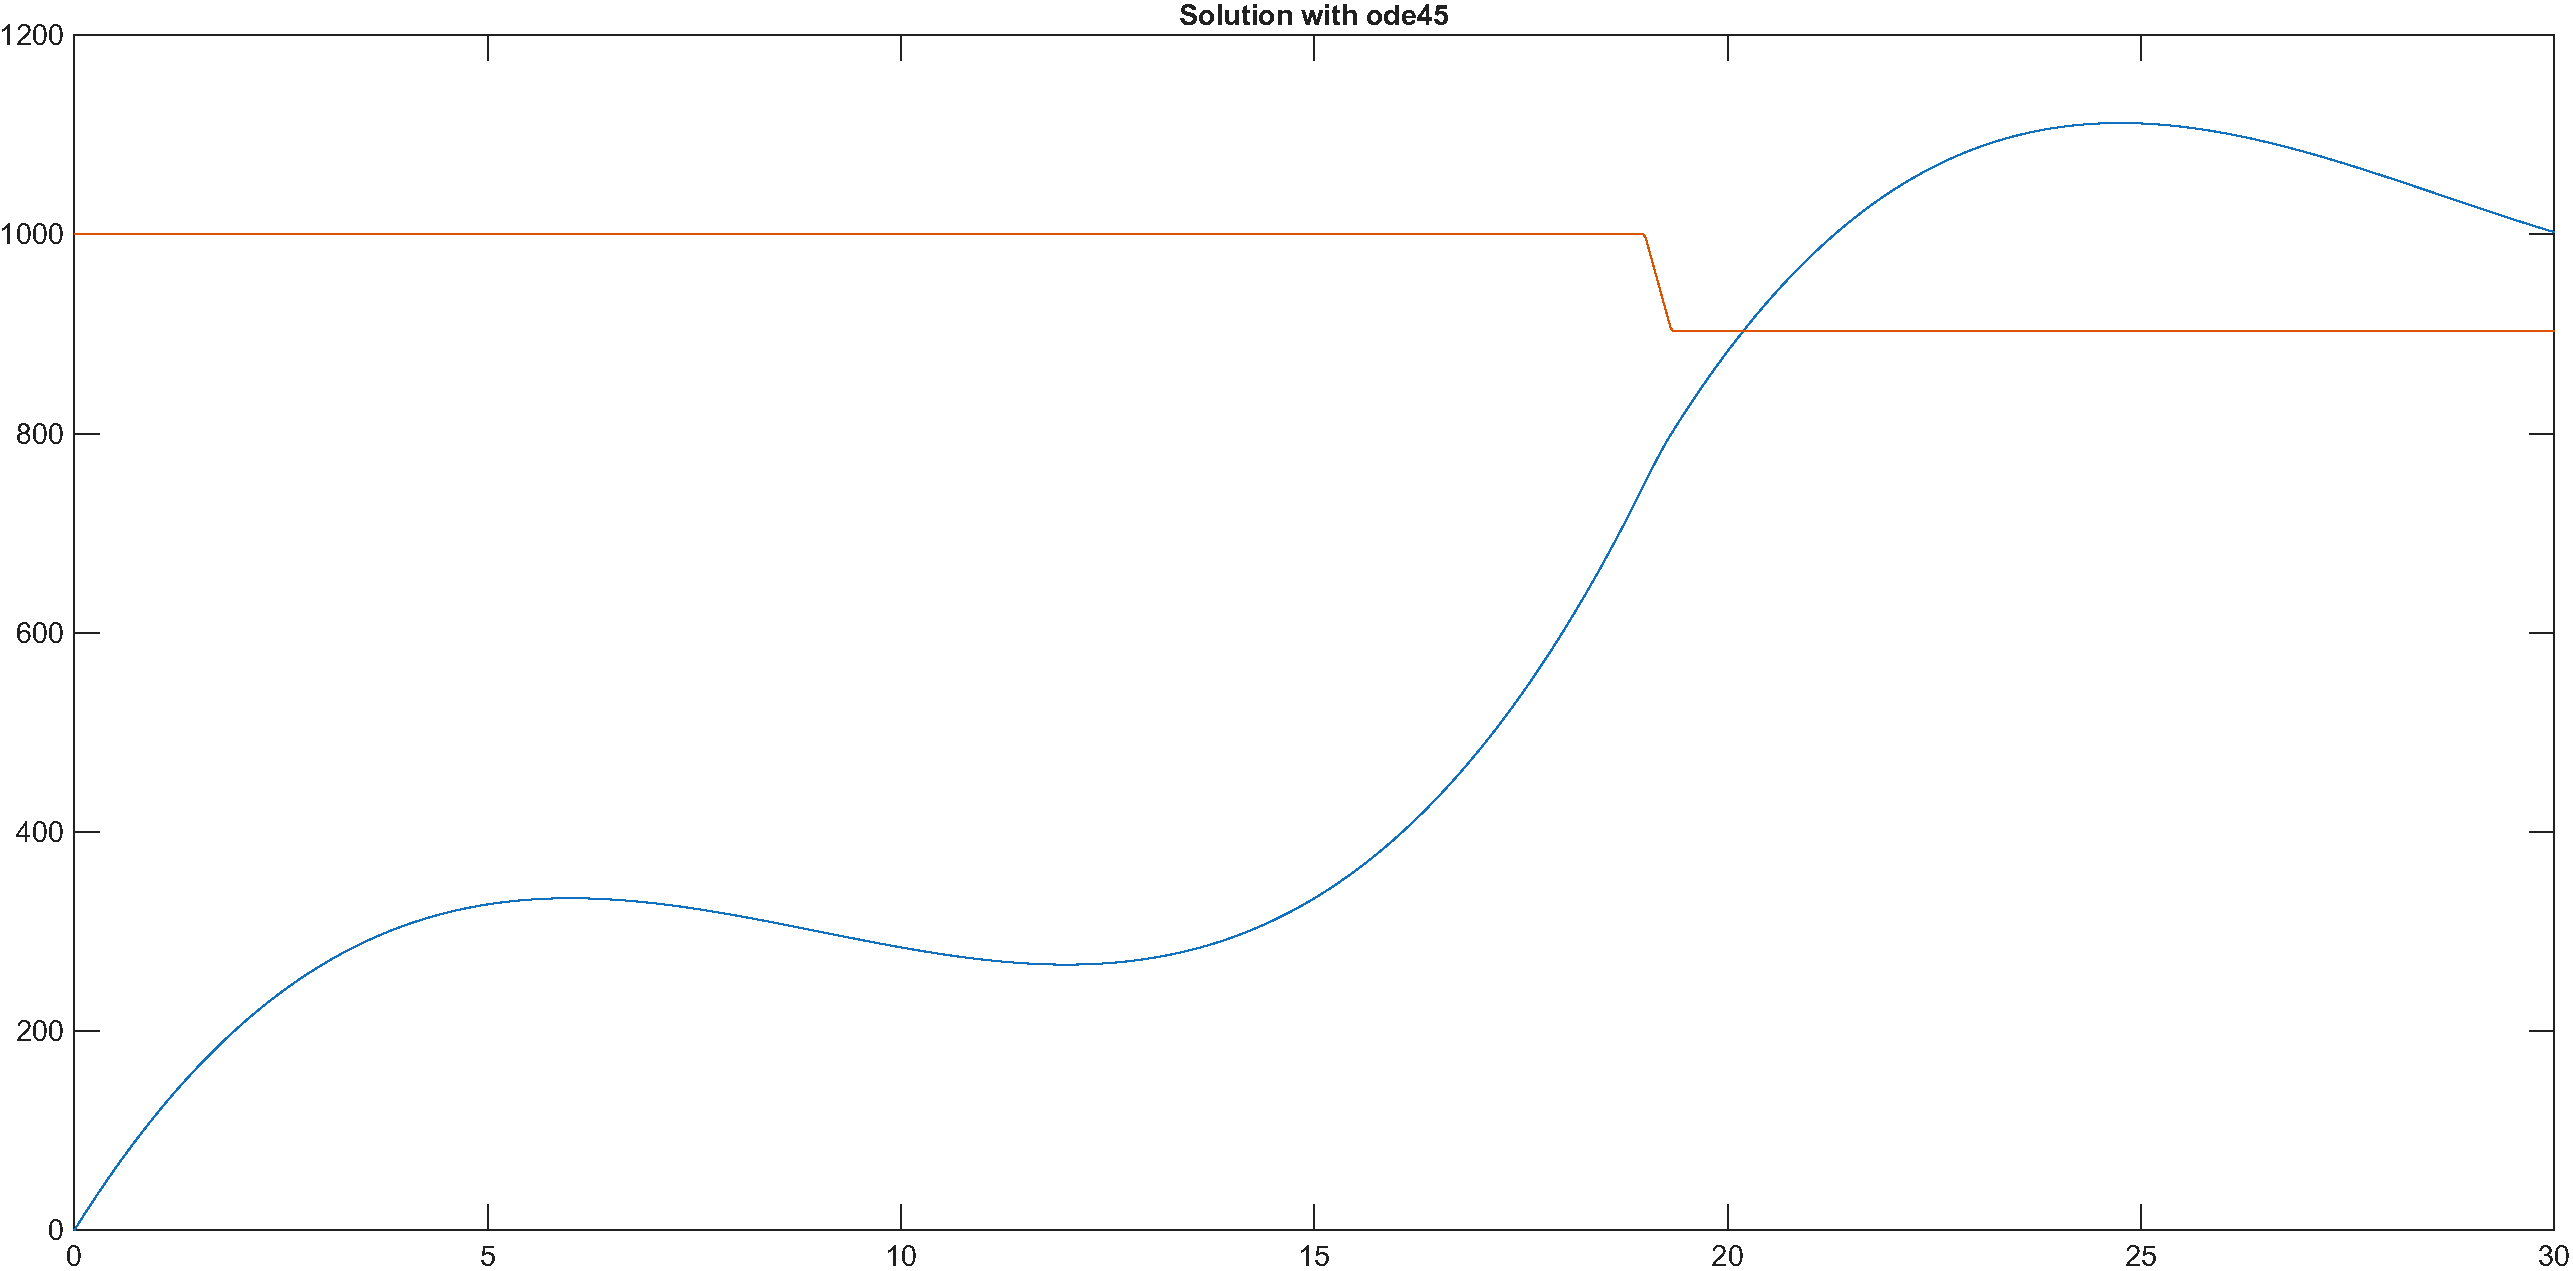
\includegraphics[width=\textwidth]{Plots/task1b}
        \caption{Solution plot with ode45 (maximum step size 0.1) for subtask \ref{item:task1b}}
    \end{figure}

    \item\label{item:task1c} The correct solution produced by IFDIFF matches the solution from subtask \ref{item:task1b}.
    
	Unlike \lstinline|ode45|, IFDIFF is designed to handle switched systems and can thus take full advantage of adaptive step size integrators like \lstinline|ode45| to compute the solution accurately and efficiently.\\\\
    \textbf{File:} \texttt{runTask1.m}
    \begin{lstlisting}
%% Subtask c)
%% Setup problem for IFDIFF
optionsIfdiff = odeset('RelTol', 1e-8, 'AbsTol', 1e-8);
datahandle = prepareDatahandleForIntegration(rhs, 'integrator', integrator, 'options', optionsIfdiff);

%% Solve with IFDIFF
solutionIfdiff = solveODE(datahandle, tspan, y0, p);

%% Plot solution
t = linspace(tspan(1), tspan(end), 1000);
yIfdiff = deval(solutionIfdiff, t);

figure;
plot(t, yIfdiff);
title('Solution with IFDIFF');
    \end{lstlisting}
    \begin{figure}[H]
        \centering
        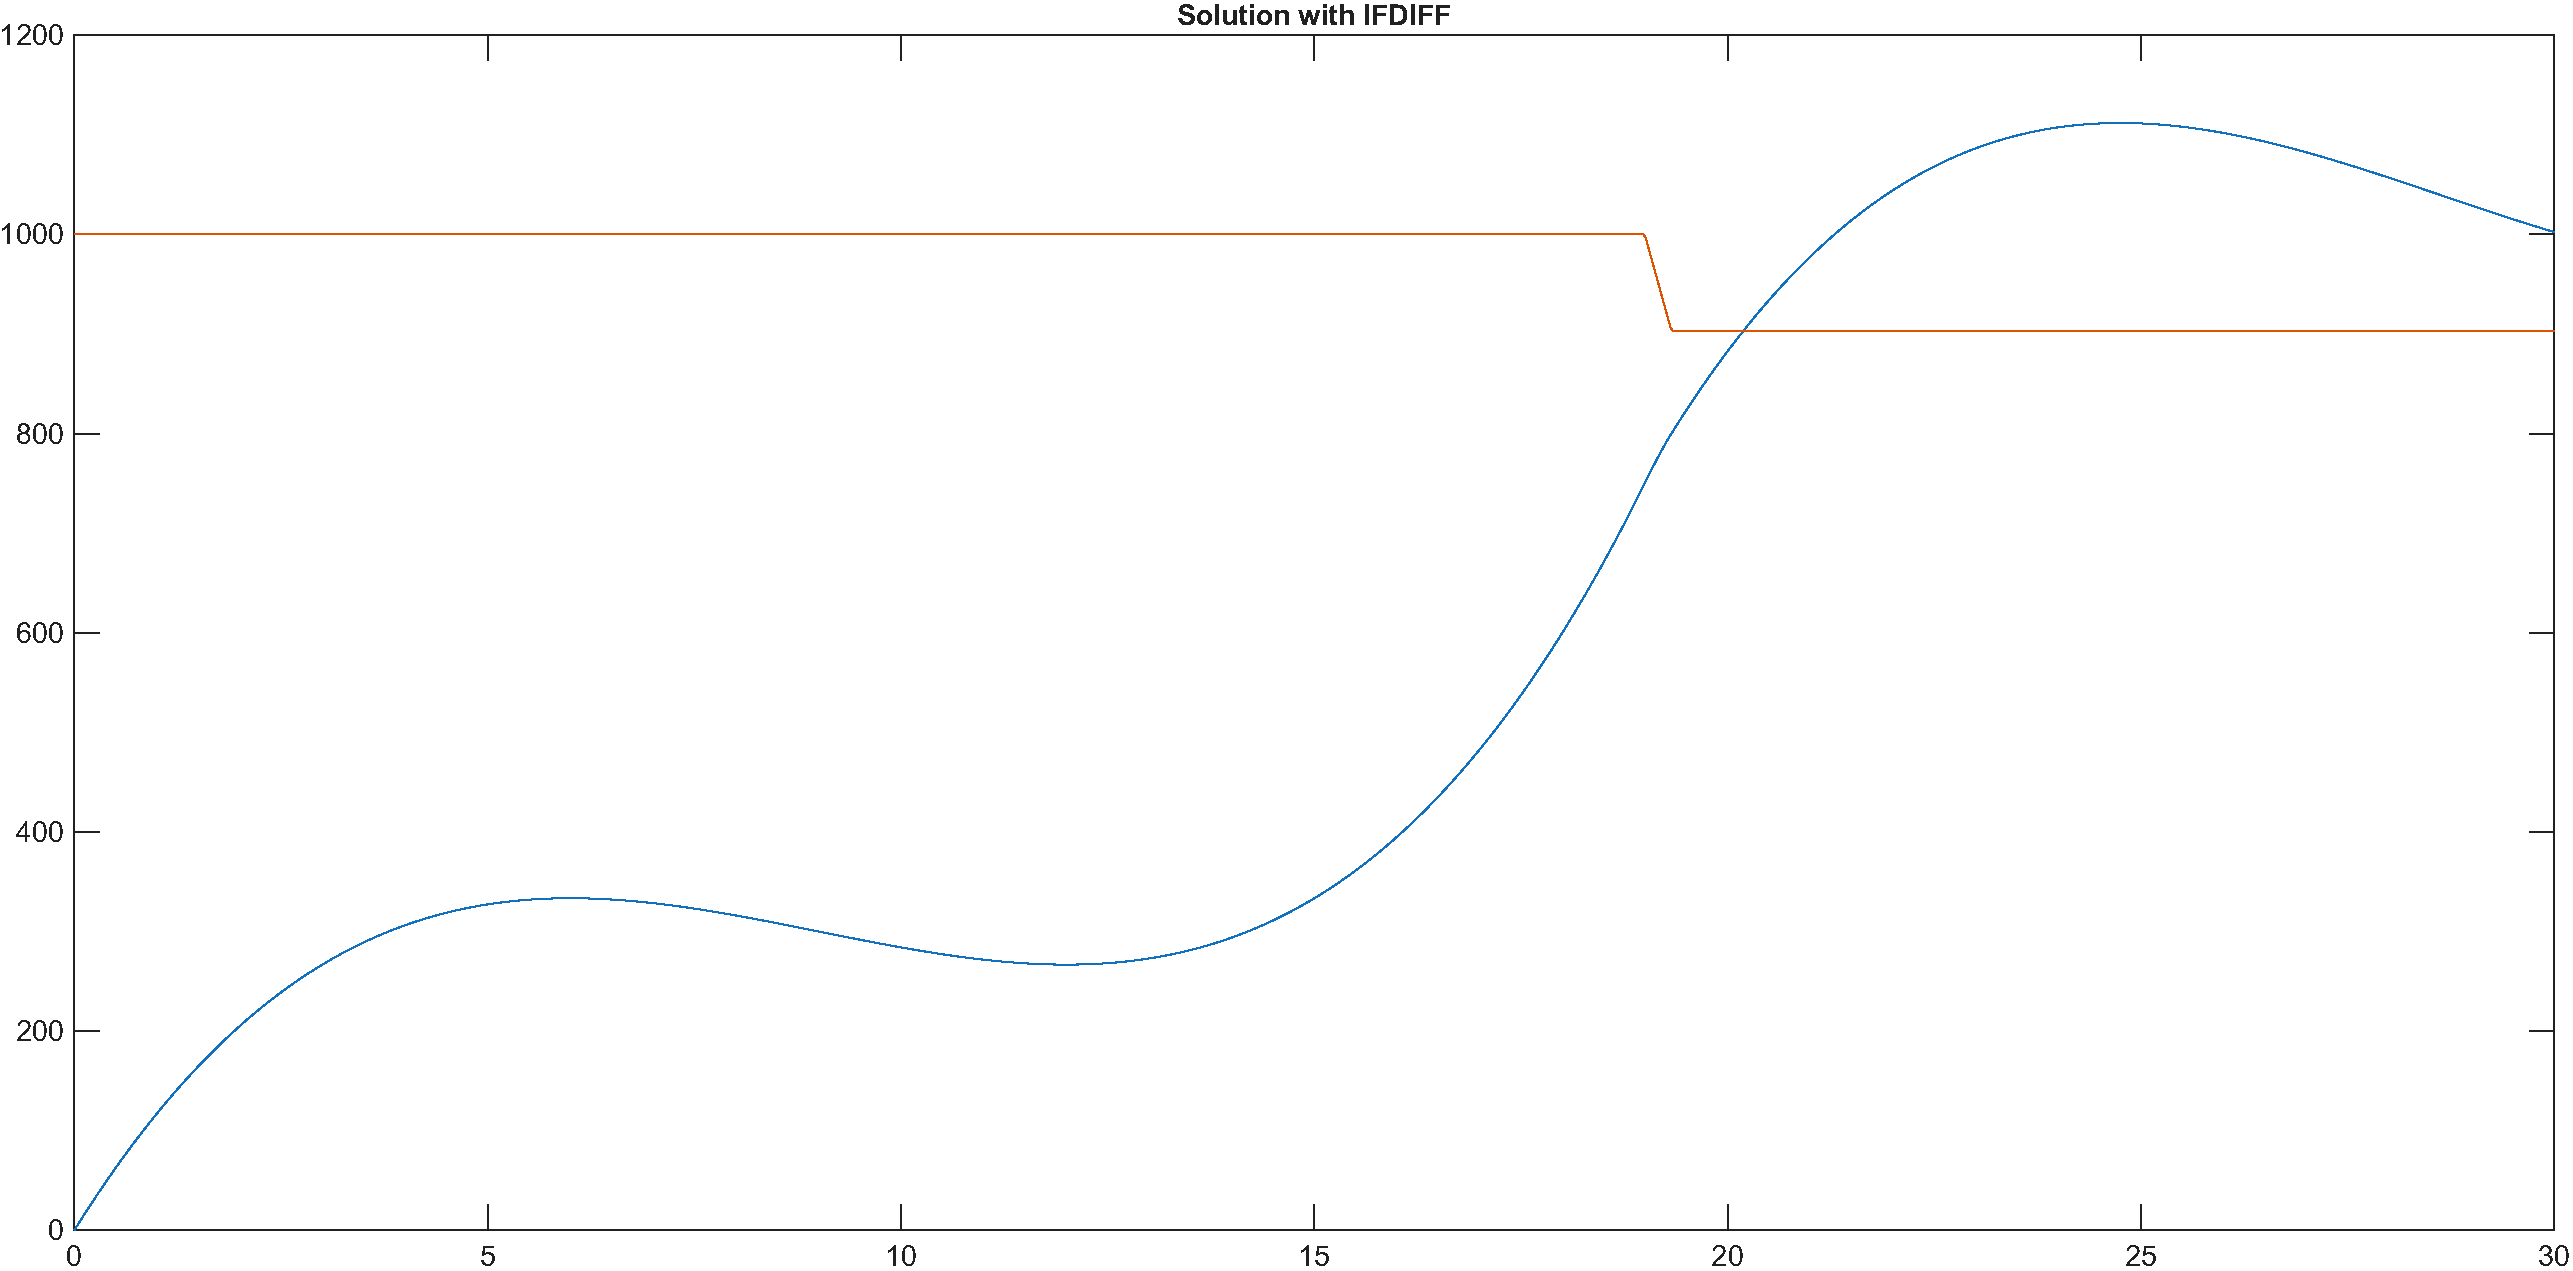
\includegraphics[width=\textwidth]{Plots/task1c}
        \caption{Solution plot with IFDIFF for subtask \ref{item:task1c}}
    \end{figure}

    \item\label{item:task1d} The sensitivities derived from the solution computed by \lstinline|ode45| are incorrect.
    
	Take $G_y(1,1)$ as an example, which describes how the first solution component changes with respect to changes in its initial value. The sensitivity before the first switch is one, which is correct because the derivative of the first solution component does not depend on the state of the first solution component, so shifting the initial value will shift the whole solution by the same amount. However, increasing the first solution component would trigger the switch earlier because $y_1(t)$ would hit the threshold $750$ quicker. Therefore, we would expect to see a sharp downwards bend in the sensitivity at the switch since the second solution component activates there and massively dampens the growth of the first solution component. This bend is completely absent in the incorrect sensitivity derived from the solution computed by \lstinline|ode45|. \\\\
    \textbf{File:} \texttt{runTask1.m}
    \begin{lstlisting}
%% Subtask d)
%% Compute sensitivity with ode45
t = linspace(tspan(1), tspan(end), 1000);
sensitivityOde45 = computeSensitivityOde45(solutionOde45, t);

%% Plot sensitivity
plotSensitivity(sensitivityOde45);
    \end{lstlisting}
    \begin{figure}[H]
        \centering
        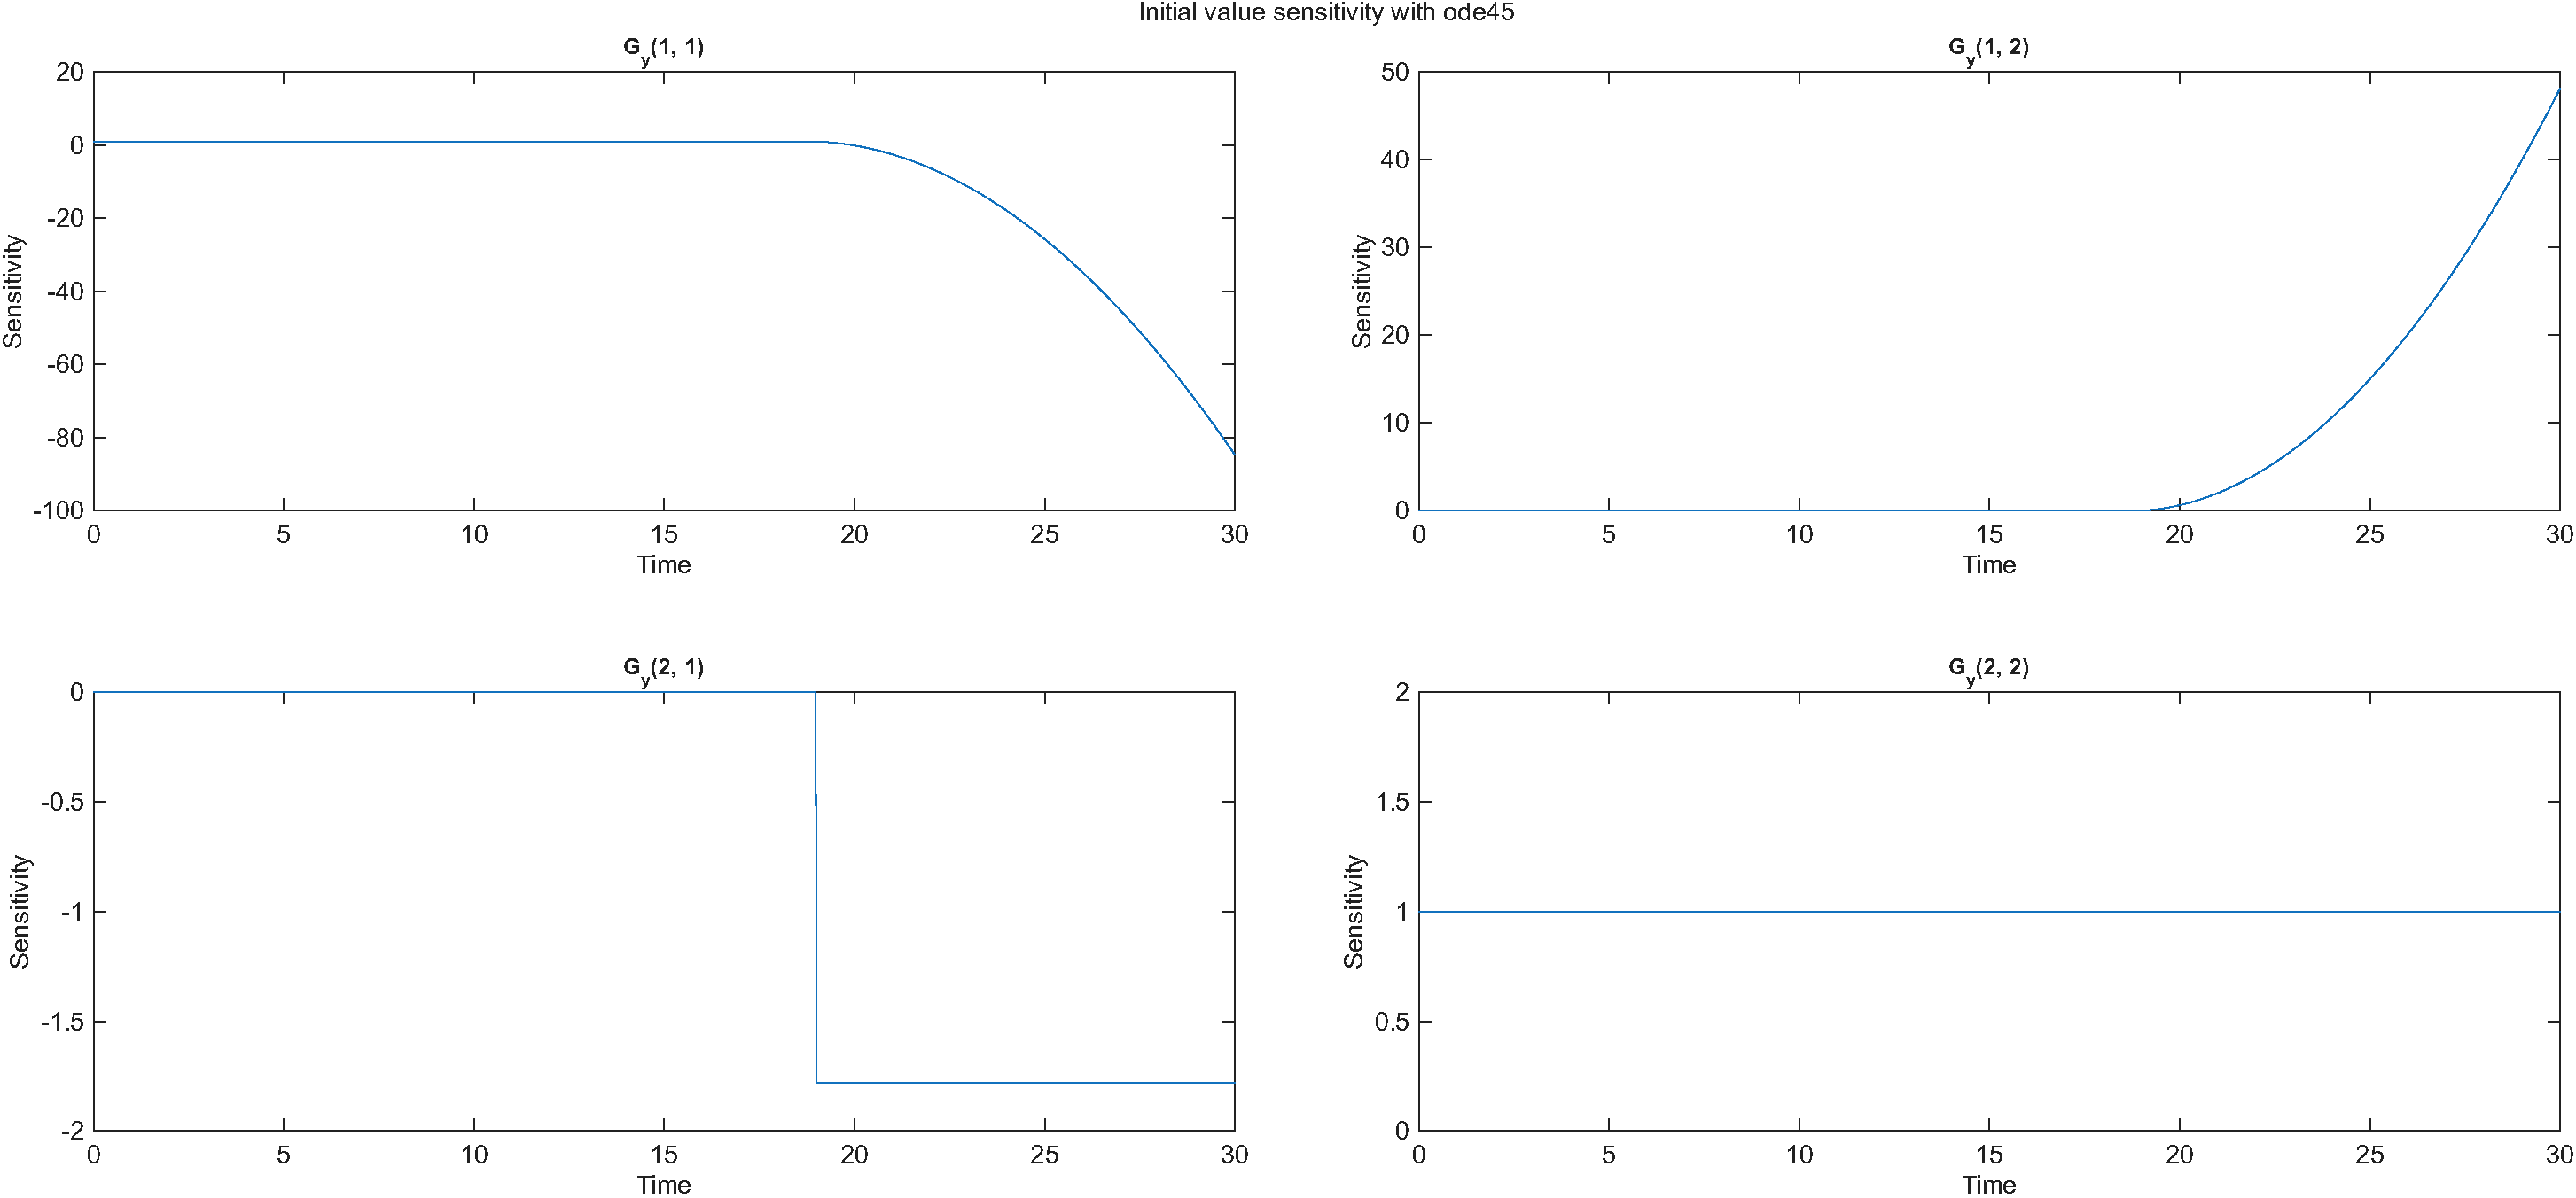
\includegraphics[width=\textwidth]{Plots/task1d}
        \caption{\textbf{Incorrect} sensitivity plot with ode45 for subtask \ref{item:task1d}}
    \end{figure}

    \item\label{item:task1e} The sensitivities computed by IFDIFF are correct.
    
	We can see the characteristic downward bend in the plot for $G_y(1,1)$, which was missing in the incorrect sensitivities from subtask \ref{item:task1d}. \\\\
    \textbf{File:} \texttt{runTask1.m}
    \begin{lstlisting}
%% Subtask e)
%% Compute sensitivity with IFDIFF
t = linspace(tspan(1), tspan(end), 1000);

sensitivityFunction = generateSensitivityFunction(datahandle, solutionIfdiff, 'calcGp', false);
sensitivityIfdiff = sensitivityFunction(t);
    \end{lstlisting}
    \begin{figure}[H]
        \centering
        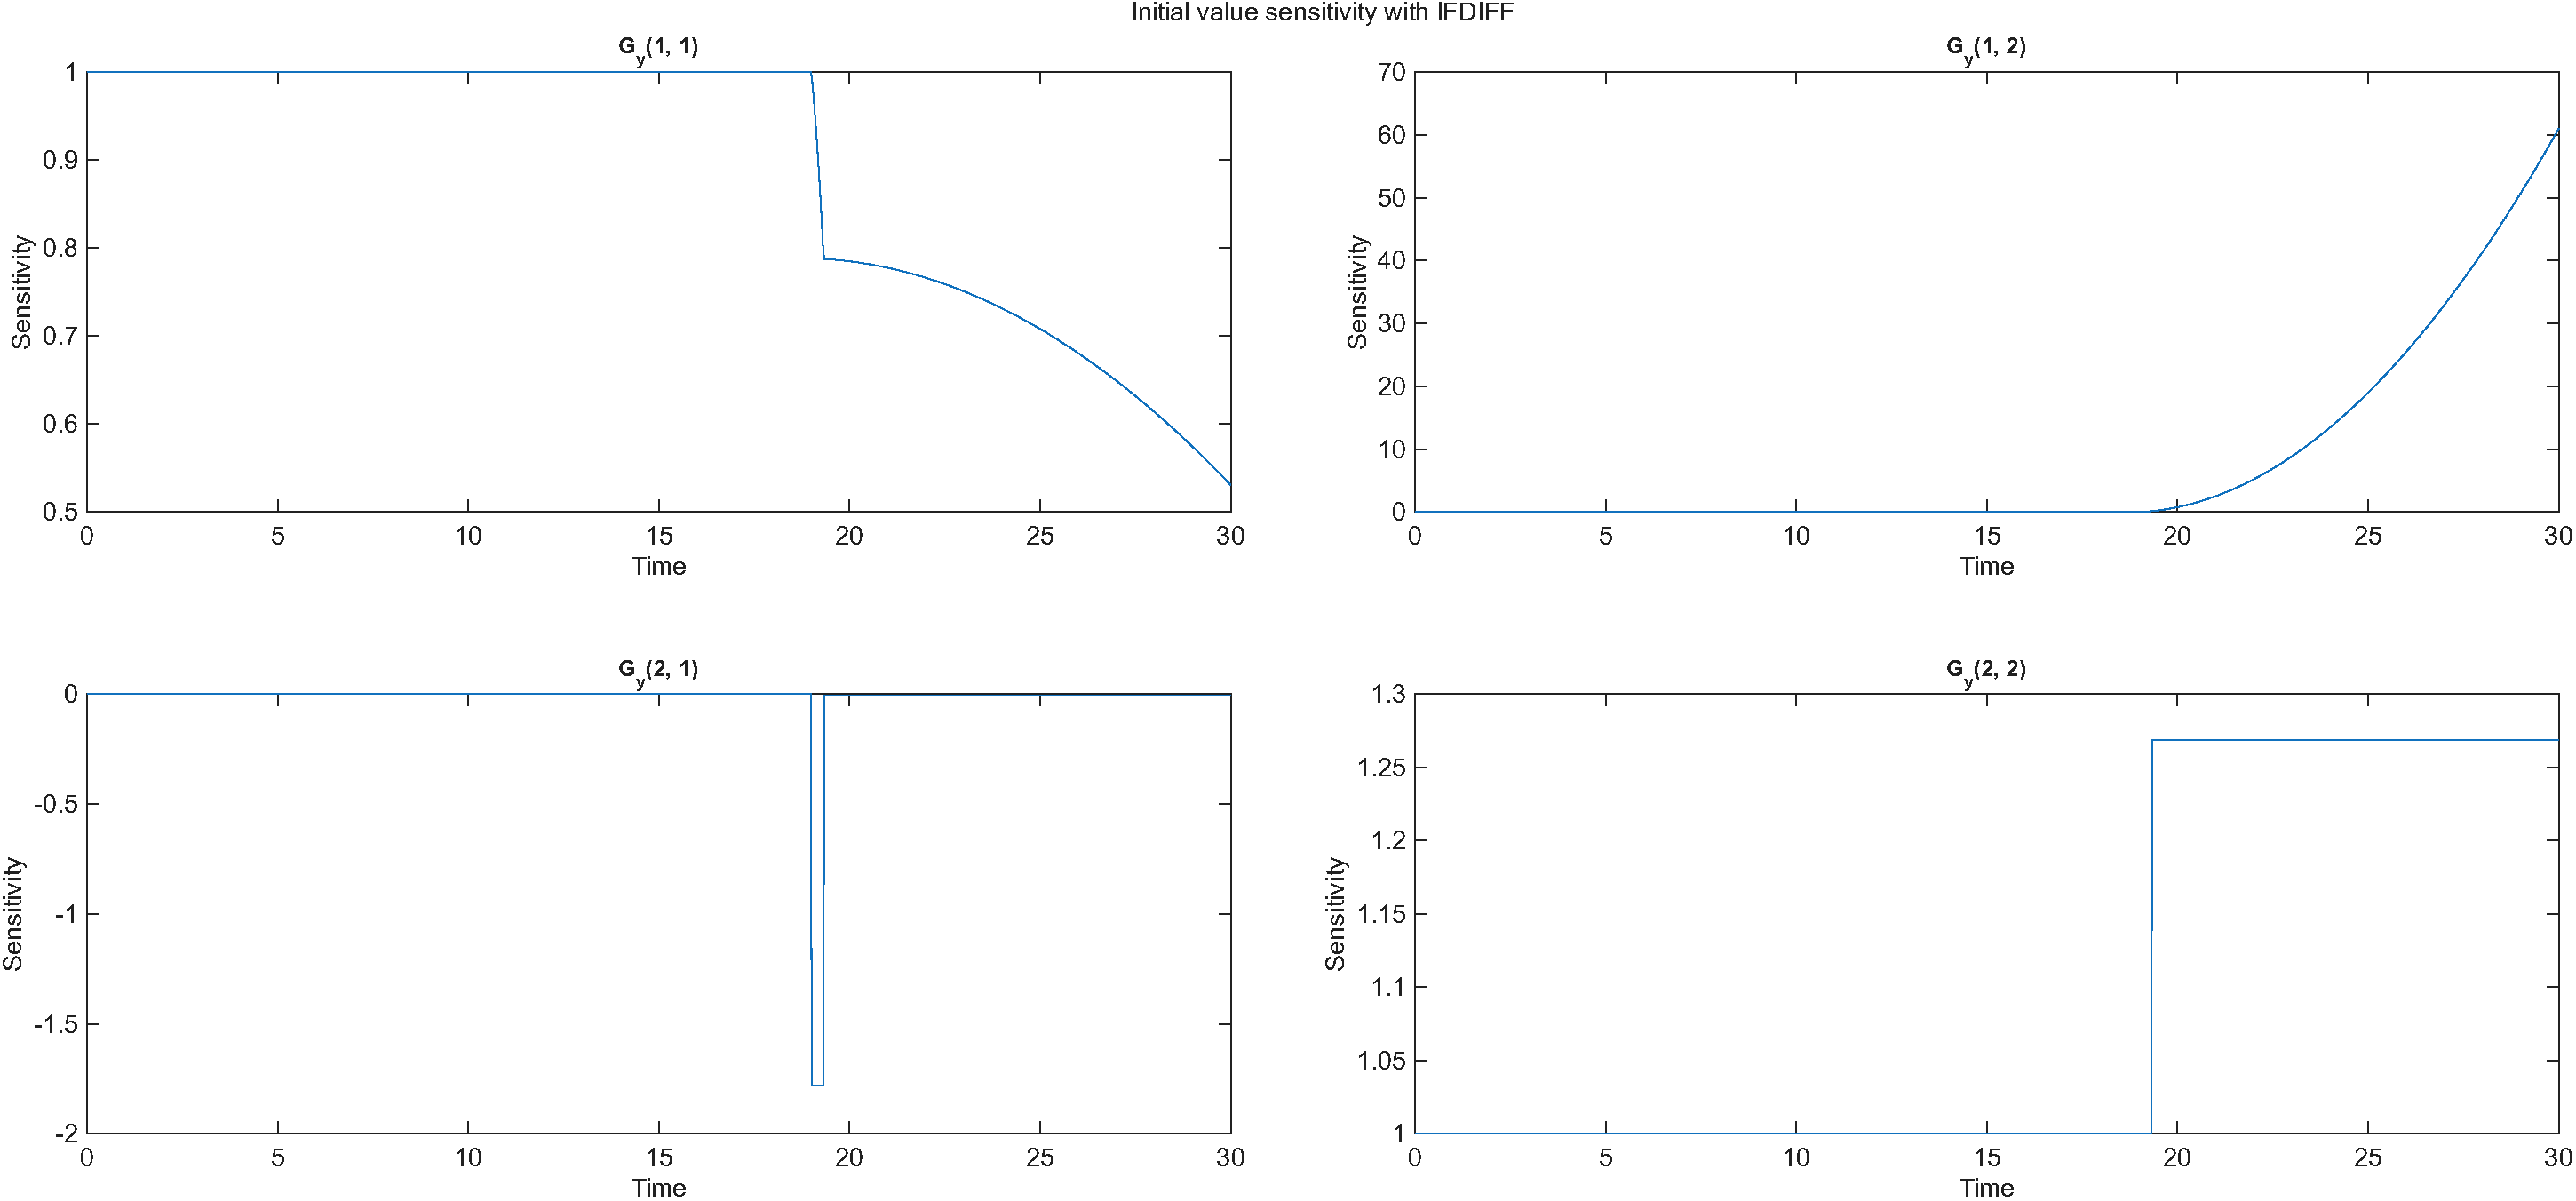
\includegraphics[width=\textwidth]{Plots/task1e}
        \caption{Sensitivity plot with IFDIFF for subtask \ref{item:task1e}}
    \end{figure}
\end{enumerate}
